\chapter{Dataset and Preprocessing}
\label{ch:dataset-preprocessing}

\section{Dataset Goal}
\label{sec:dataset-goal}

The goal of the dataset is to evaluate malicious-bitstream inspection on the same type of artifact that appears in a serverless FPGA deployment path. The input to the checker is a partial bitstream, not source code, a netlist, or an implementation report. The dataset is therefore built from Coyote-style partial bitstreams.

The classification task is binary. Benign samples are partial bitstreams generated from Coyote applications. Malicious samples are partial bitstreams that contain ring-oscillator payloads. Labels are assigned by construction from the generation flow.

This dataset is designed to test deployment-like variation. Samples are generated across different floorplans and configurations so that the classifier is not evaluated on a single fixed placement. The malicious class also includes higher-density RO samples to evaluate how detection changes as the RO footprint increases.

\section{Bitstream Generation}
\label{sec:bitstream-generation}

Benign samples are generated from real Coyote applications. These applications represent normal user accelerators that could be deployed into a reconfigurable region. To increase variation, the applications are built across multiple floorplans and configurations.

The benign catalog contains eight debug-enabled Coyote applications: hello world, HLS vector add, multitenancy AES, user interrupts, perf FPGA, multithreading AES, Euclidean distance, and cosine similarity. It also contains no-debug variants for seven of these applications. In the available manifests, this gives 120 debug-enabled benign samples and 101 no-debug benign samples.

Malicious samples are generated from RO-based designs. These designs place attacker-controlled ring oscillators into the reconfigurable region. The RO count is varied to create payloads with different logic footprints. This allows the evaluation to distinguish between small low-footprint payloads and larger high-density payloads.

Figure~\ref{fig:dataset-pipeline} shows the dataset generation flow. Both benign and malicious designs pass through the same floorplan and configuration sweep before partial-bitstream generation. The output is a labeled dataset of partial bitstreams and metadata.

\begin{figure}[t]
    \centering
    % Figure generated locally from figures/dataset_generation_pipeline.dot.
    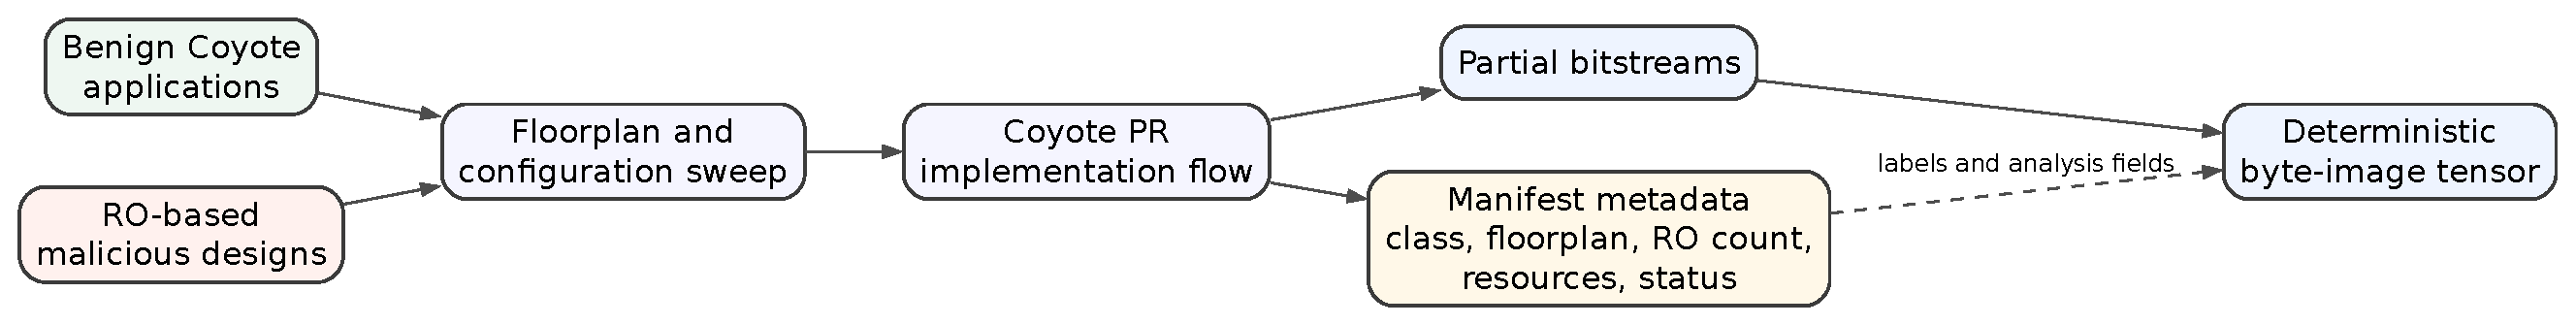
\includegraphics[width=0.95\linewidth]{figures/dataset_generation_pipeline.pdf}
    \caption{Dataset generation pipeline. Benign Coyote applications and RO-based malicious designs are generated across deployment-like variation and converted into labeled partial bitstreams.}
    \label{fig:dataset-pipeline}
\end{figure}

\section{Dataset Composition}
\label{sec:dataset-composition}

Table~\ref{tab:dataset-composition} summarizes the available generated dataset. The original generated corpus contains benign Coyote bitstreams and normal-RO malicious bitstreams across 15 floorplans, FP00--FP14. The higher-density big-RO extension uses six of those floorplans and is kept separate because it is used for the extended footprint evaluation.

The available generated manifests contain 221 benign samples, 225 normal-RO malicious samples, and 78 big-RO malicious samples. The normal-RO corpus spans 33 RO-count settings. The big-RO extension spans 13 higher-density RO-count settings.

\begin{table}[t]
    \centering
    \caption{Dataset composition by class and RO category.}
    \label{tab:dataset-composition}
    \small
    \resizebox{\linewidth}{!}{
    \begin{tabular}{@{}l l l r r@{}}
        \toprule
        \textbf{Class} & \textbf{Source} & \textbf{Variation} & \textbf{Floorplans} & \textbf{Samples} \\
        \midrule
        % Sources: ../ml_deep_bitstream_inspection/datasets/full_dataset_it{1,2,3}/artifacts/manifest_available.csv
        Benign &
        Coyote applications &
        8 apps, 7 no-debug variants &
        15 &
        221 \\
        \midrule
        % Sources: ../ml_deep_bitstream_inspection/datasets/full_dataset_it{1,2,3}/artifacts/manifest_available.csv
        Normal RO &
        Standalone RO payloads &
        33 RO-count settings &
        15 &
        225 \\
        \midrule
        % Source: ../ml_deep_bitstream_inspection/datasets/full_dataset_it4_big_ro/artifacts/manifest_available.csv
        Big RO &
        Higher-density RO payloads &
        13 RO-count settings &
        6 &
        78 \\
        \bottomrule
    \end{tabular}
    }
\end{table}

Each sample also stores metadata used during analysis. This includes the design source, floorplan, configuration, label, bitstream size, and estimated RO footprint when applicable. The RO footprint metadata is used later to evaluate whether misses concentrate in small malicious designs.

\section{Preprocessing}
\label{sec:preprocessing}

The preprocessing step converts each partial bitstream into the fixed input shape expected by the CNN. The transform is intentionally simple. It does not reverse-engineer the bitstream. It does not extract hand-crafted circuit features. It treats the partial bitstream as a byte stream.

Each bitstream is read as a sequence of bytes
\[
    b = [b_0, b_1, \ldots, b_n].
\]
The sequence is resized to a fixed number of bytes. If the bitstream is longer than the target size, it is downsampled. If it is shorter, it is padded. The result is reshaped into a grayscale image-like tensor.

The main input resolutions are
\[
    128^2,\quad 256^2,\quad 512^2.
\]
Larger resolutions are also used during model exploration to measure how much classification quality improves when more bitstream detail is preserved.

This representation is useful for two reasons. First, it gives CNNs a fixed-size input while preserving byte-level structure from across the bitstream. Second, the operation is simple enough to implement in FPGA logic before inference. This matters because the final goal is an FPGA-resident checker that can run in the deployment path.

\section{Dataset Limitations}
\label{sec:dataset-limitations}

The dataset supports a feasibility study. It does not cover every malicious FPGA design. The malicious class focuses on RO-based payloads, and labels are assigned by construction. This means the classifier may learn artifacts that correlate with maliciousness, such as payload size, routing density, or floorplan effects.

The extended RO-footprint evaluation helps address this issue by showing where the detector is strong and where it is weak. Small RO payloads remain the harder case. Larger RO payloads are more relevant for power-stress attacks and are evaluated separately in Section~\ref{ch:cnn-pipeline}.
